\documentclass[10pt,preprint]{aastex}
\usepackage{amsmath}
\usepackage{breqn}
\usepackage{cite,natbib}
\usepackage{natbib}
\usepackage{epsfig}
\usepackage{cases}
\usepackage[section]{placeins}
\usepackage{graphicx, subfigure}
\usepackage{color}
\usepackage{amsmath}
\usepackage{float}
\floatplacement{figure}{H}
% \usepackage[nomarkers,figuresonly]{endfloat}

\newcommand{\logg}{log \emph{g}~}
\newcommand{\teff}{$T_{eff}~$}
\newcommand{\prot}{$P_{rot}~$}

\newcommand{\ah}{$\hat{A}_n$}
\newcommand{\ph}{$\hat{P}_n$}
\newcommand{\ch}{$\hat{C}_n$}
\newcommand{\gh}{$\hat{G}_n$}
\newcommand{\yh}{$\hat{Y}_n$}
\newcommand{\teffh}{$\hat{T}_n$}

\newcommand{\feh}{[Fe/H]}
\newcommand{\dd}{\ensuremath{\,\mathrm{d}}}

\begin{document}

\citet{Garcia2014} use a combination of wavelet transforms and ACFs to measure the surface rotation periods of Kepler asteroseismic stars.
They use a Morlet mother wavelet which is the convolution of a sinusoid and a Gaussian.
They require that at least four full rotation periods are present in the data
They use two sets of data: PDC-MAP and KADACS and two periodicity measurement methods: ACF and wavelet transform.
They require all four of these possible data and analysis method combinations to be consistent to within 20\%.
They then visually check the data.
compute a wavelet transform for each light curve and project it onto the period axis, reinforcing the true period and suppresing harmonic and sub-harmonic signals.
The details of this method are outlined in \citet{Mathur2014}.

\subsection{Supplementary data}

The asteroseismic sample covers a large range of ages (see figure \ref{fig:p_vs_a}), however it does not provide good mass coverage at all ages.
There are very few stars with temperatures below 6000 K (B-V $\sim$ 0.55) and of the low mass stars, most of them are old.
We therefore added 260 stars to our sample from young clusters Coma Berenices (0.5 Gyr), Praesepe (0.588 Gyr), the Hyades (0.625 Gyr) and NGC6811 (1.1 Gyr) (see table \ref{tab:clusters}).
We did not add clusters aged less than 0.5 Gyrs as these often have large populations of rapid rotators that have not yet converged onto the gyrochronology plane.

\begin{deluxetable}{lccc}
\label{tab:clusters}
\tablewidth{0pc}
\tablecaption{Clusters and References: (1) \citet{Soderblom2009}, (2) \citet{Hartman2010}, (3) \citet{Jones1996}, (4) \citet{Meibom2011_M34}, (5) \citet{Dobbie2009}, (6) \citet{CollierCameron2009}, (7) \citet{Khalaj2013}, (8) \citet{Kovacs2014}, (9) \citet{Perryman1998}, (10) \citet{Radick1987}, (11) \citet{Janes2011}, (12) \citet{Meibom2011}. NGC 6811 g-r colours were converted to dereddened B-V with $E_{(B-V)}$ = 0.1. The age of M 34 reported in \citet{Jones1996} is 200-250 Myr.}
\tablehead{
\colhead{Cluster}&
\colhead{Age (Gyr)}&
\colhead{Age ref}&
\colhead{Rotation period ref}}
\startdata
% Pleides & 0.1 $\pm$ 0.05 & 1 & 2 \\
% M 34 & 0.225 $\pm$ 0.025 & 3 & 4 \\
Coma Ber & 0.5 $\pm$ 0.1 & 5 & 6 \\
Praesepe & 0.588 $\pm$ 0.137 & 7 & 8 \\
Hyades & 0.625 $\pm$ 0.05 & 9 & 10 \\
NGC 6811 & 1.1 $\pm$ 0.2 & 11 & 12 \\
\enddata
\end{deluxetable}

\begin{deluxetable}{lccc}
\label{tab:field_stars}
\tablewidth{0pc}
\tablecaption{Rotation periods and B-V colours for field stars with precise ages.
References: (1) \citet{Metcalfe2012}, (2) \citet{Henry2000}, (3) \citet{Moffet1979}, (4) \citet{Li2012}, (5) \citet{Petit2008}, (6) \citet{Mermilliod1986}, (7) \citet{Bouvier2010}, (8) \citet{Donahue1996}, (9) \citet{Cox2000}, (10) \citet{Bazot2012}, (11) \citet{Yildiz2007}, (12) \citet{Hallam1991}, (13) \citet{Dumusque2012}.}
\tablehead{
\colhead{ID}&
\colhead{age}&
\colhead{\prot}&
\colhead{B-V}}
\startdata
16 Cyg B & 6.4 $\pm$ 0.4$^1$ & 31.5 $\pm$ 6.5$^2$ & 0.66 $\pm$ 0.01$^3$ \\
18 Sco & 3.66 $\pm$ 0.2$^4$ & 22.7 $\pm$ 0.5$^5$ & 0.64 $\pm$ 0.01$^6$ \\
The Sun & 4.568 $\pm$ 0.001$^7$ & 26.09 $\pm$ 0.1$^8$ & 0.65 $\pm$ 0.001$^9$ \\
$\alpha$ Cen A & 6 $\pm$ 1$^{10,11}$ & 28.8 $\pm$ 2.5$^{12}$ & 0.69 $\pm$ 0.01$^6$ \\
$\alpha$ Cen B & 6 $\pm$ 1$^{10,11}$ & 38.7 $\pm$ 5.0$^{13}$ & 0.90 $\pm$ 0.01$^6$ \\
\enddata
\end{deluxetable}

\begin{figure}[ht]
\begin{center}
	\subfigure[$P_{rot}$ vs \teff]{
            \label{fig:p_vs_t}
	    \includegraphics[width=3in, clip=true, trim=0 0 0.5in 0]{/Users/angusr/Python/Gyro/plots/p_vs_t_paper.png}
        }
	\subfigure[$P_{rot}$ vs B-V colour]{
            \label{fig:p_vs_bv}
	    \includegraphics[width=3in, clip=true, trim=0 0 0.5in 0]{/Users/angusr/Python/Gyro/plots/p_vs_bv_paper.png}
        }
    \end{center}
    \caption{ Photometric rotation period vs effective temperature and B-V colour for 153 Kepler asteroseismic targets. \teff was converted to B-V using \citet{Sekigchi2000}.
     }
   \label{fig:subfigures}
\end{figure}

Rotation periods and B-V colours for the Hyades were obtained from \citet{Radick1987} and an age of 650 Myrs was adopted from \citet{Perryman1998}.
NGC 6811 is a cluster in the Kepler field with an age of 1.1 $\pm$ 0.2 Gyr \citep{Janes2011} with photometric rotation periods for cluster members measured by \citet{Meibom2011}.
These stars have g-r colours which were converted to dereddened B-V with $E_{(B-V)} = 0.1$.
Rotation periods for the 590 Myr \citep{Khalaj2013} cluster Praesepe were published in \citet{Kovacs2014}, with B and V colours from the APASS database ((http://www.aavso.org/apass).

A further 5 field stars with precise age measurements were added to the sample: 16 Cyg B, Alpha Cen A and B, 18 Sco and, of course, the Sun (see table \ref{tab:field_stars}).
An asteroseismic age for 16 Cyg B was obtained from \citet{Metcalfe2012}, $T_{eff}$ from \citet{Ramirez2009} and rotation period from \citet{Henry2000} with B and V colours from \citet{Moffett1979}.
An age of 6 $\pm$ 1 Gyr was adopted for Alpha Cen AB, based on the analysis by \citet{Bazot2012} and \citet{Yildiz2007} (note that ages derived for Alpha Cen AB are extremely model dependent).
B and V colours were obtained from \citet{Mermilliod1986} and rotation periods from \citet{Hallam1991} and \citet{Dumusque2012} for A and B, respectively.
An age of 4.568 $\pm$ 0.001 Gyr for the Sun was taken from \citet{Bouvier2010}, and a latitudinal mean rotation period, observed by \citet{Donahue1996}.
% We also include the Sun as an old anchor datum, adopting a period of 26.09 days which is the latitudinal mean observed by Donahue et al. (1996) (the solar rotation ranges from ø25 days near the equator to ø32 days near the poles).
The age of 3.66 $\pm$ 0.2 for 18 Sco was taken from \citet{Li2012}, with rotation period from \citet{Petit2008} and B and V colours from \citet{Mermilliod1986}.

Despite having effective temperatures for the asteroseismic targets, we converted $T_{eff}$ to B-V colours, using the relation in \citet{Sekiguchi2000}---see figure \ref{fig:subfigures}.
This conversion is imprecise since the metallicites of the asteroseismic targets are the field average and not calculated per star.
Eventually we intend to provide an effective temperature calibration in addition to this colour calibration.
% however we concluded that converting $T_{eff}$ to colour would be more efficient than converting cluster star colours to $T_{eff}$, since we have more information about the asteroseismic sample.

The entire set of 418 stars is shown in figure \ref{fig:3d}. Asteroseismic targets are shown in black, with supplementary cluster and field stars in red.

\begin{figure}[ht]
\begin{center}
\includegraphics[width=6in, clip=true, trim=0 0 0.5in 0]{/Users/angusr/Python/Gyro/plots/3d_angled.png}
\caption{Colour, age and rotation periods of all 418 stars. Asteroseismic stars are black and additional cluster and field stars are red. {\color{red}add precise stars.}}
\label{fig:3d}
\end{center}
\end{figure}

\begin{figure}[ht]
\begin{center}
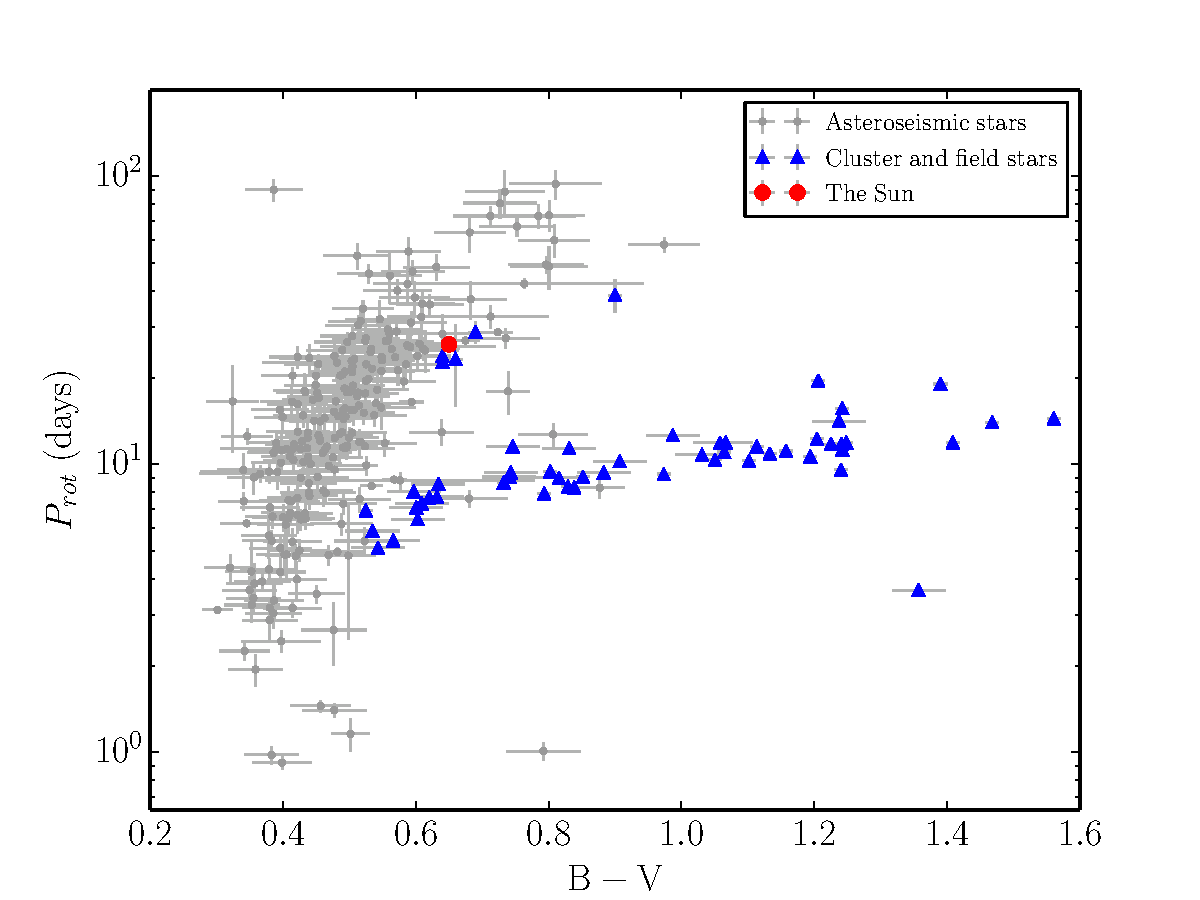
\includegraphics[width=6in, clip=true, trim=0 0 0.5in 0]{/Users/angusr/Python/Gyro/plots/p_vs_bv_paper2.png}
\caption{Photometric rotation period vs B-V colour for 153 Kepler targets (black) plus cluster and field stars (red). The blue stars have precise ages.}
\label{fig:3d}
\end{center}
\end{figure}

\begin{figure}[ht]
\begin{center}
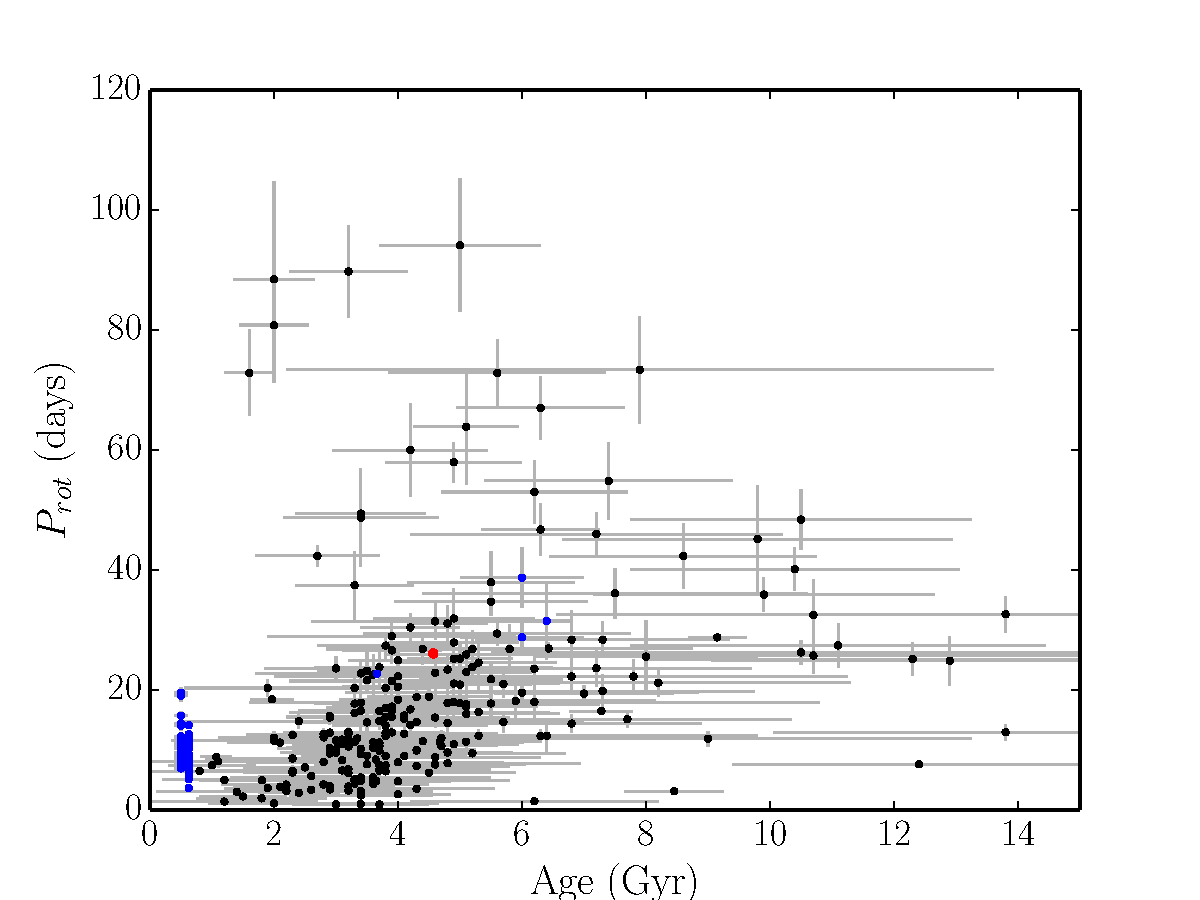
\includegraphics[width=6in, clip=true, trim=0 0 0.5in 0]{/Users/angusr/Python/Gyro/plots/p_vs_a_paper2.png}
\caption{Photometric rotation period vs age for 153 Kepler targets (black) plus cluster and field stars (red). The blue stars have precise ages. {\color{red} add 7 other precise stars.}}
\label{fig:p_vs_a}
\end{center}
\end{figure}

\bibliographystyle{plainnat}
\bibliography{Gyro_paper}

\end{document}
